\documentclass[openany, notitlepage, justified]{tufte-book}
\usepackage{amsmath, amssymb, amsthm}
\usepackage{graphicx, epsdice}

\geometry{                                                                      
    height=11.0in,                                                              
    width=8.5in,                                                                
    left=1in, % left margin                                                     
    textwidth=5.0in, % main text block                                          
    marginparsep=0.2in, % gutter between main text block and margin notes       
    marginparwidth=1.8in % width of margin notes                                
}    

\usepackage{etoolbox}
\makeatletter
\patchcmd{\chapter}{\if@openright\cleardoublepage\else\clearpage\fi}{}{}{}
\makeatother

\newcommand{\EE}{\mathbb{E}}
\newcommand{\PP}{\mathbb{P}}
%
\newcommand{\Dd}{\mathcal{D}}
\newcommand{\Ee}{\mathcal{E}}
\newcommand{\Gg}{\mathcal{G}}
\newcommand{\Hh}{\mathcal{H}}
\newcommand{\Ii}{\mathcal{I}}
\newcommand{\Ll}{\mathcal{L}}
\newcommand{\Ss}{\mathcal{S}}
\newcommand{\Xx}{\mathcal{X}}
\newcommand{\Yy}{\mathcal{Y}}

\newcommand{\sdia}[1]{
\begingroup
\setbox0=\hbox{\includegraphics[height=\baselineskip]{#1}}%
\parbox{\wd0}{\box0}\endgroup
}

\begin{document}

    \begin{adjustwidth}{0in}{-1.9in}
    \begin{center}
        \Huge 
        Generalization in Machine Learning \\
        \large         
        Sam, Joe, and Arthur ~~~~~~~~~~ 2020 Summer
    \end{center}
    \end{adjustwidth}

    \chapter{The Cake Problem}
        \section{A Tempting Pattern}
            We'll start out with a fun puzzle that's not directly related to
            machine learning but whose math will later help us.
            %
            Imagine $n$ people are seated around a large disk-shaped cake.
            Each pair of people will use a two-person handsaw to cut the cake.
            For example, the picture below shows a group of $4$ people; there
            are $6$ pairs of people, so the group makes $6$ cuts total.  When
            $4$ people encircle the cake, it ends up cut into $8$ pieces.  We
            wonder: how many pieces arise when a different number of people sit
            around the cake?
            %
            \begin{marginfigure}
                \centering
                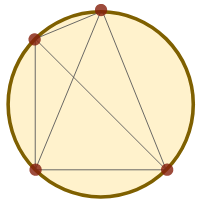
\includegraphics[height=3cm]{cake-4}
                \caption{\emph{
                    With $n=4$ people, we make ${n\choose 2}=6$ cuts, which gives
                    $8$ pieces in total ($4$ outside and $4$ inside).  
                }}
            \end{marginfigure}

            Here are some drawings for possibilities ranging from $n=1$ people
            to $n=6$ people.  Try counting the pieces and guessing a pattern!
            Can you find a formula for how many pieces arise when there are $n$
            people?
            \begin{figure}[h!]
                \centering
                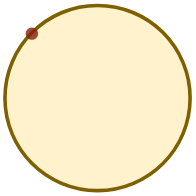
\includegraphics[height=3cm]{cake-1}
                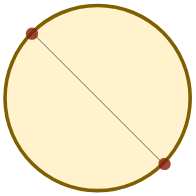
\includegraphics[height=3cm]{cake-2}
                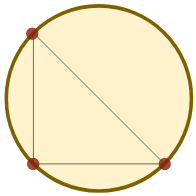
\includegraphics[height=3cm]{cake-3} \\
                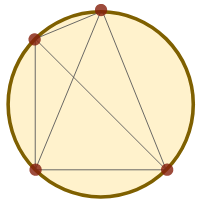
\includegraphics[height=3cm]{cake-4}
                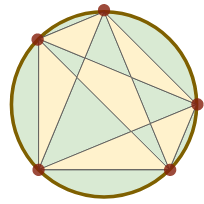
\includegraphics[height=3cm]{cake-5-col}
                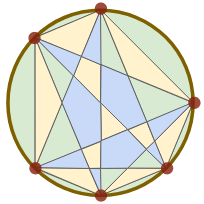
\includegraphics[height=3cm]{cake-6-col}
                \caption{\emph{
                    Here, we color some of the cake pieces just to make them
                    easier to see and to count.
                    %
                    The $n=1$ case doesn't have any cuts.
                    %
                    The $n=5$ case has $5$ outside green pieces, $5$ inside
                    green pieces, $5$ yellow triangles --- so far this is three
                    fives, which makes fifteen --- and what's left is $1$
                    yellow center piece.
                    %
                    The $n=6$ case has $6$ outside green pieces, $6$ inside
                    green pieces, $6$ outer yellow triangles, $6$ blue
                    triangles --- so far this is four sixes, which makes twenty
                    four --- and what's left are the $7$ central blue and
                    yellow shapes.
                }}
            \end{figure}

            Well, it seems that with $n=1, 2, 3, 4$ people, there are $p(n) =
            1, 2, 4, 8$ pieces.  (Here, $p$ stands for ``pieces'', and we'll
            use this way of writing just to save time).  It seems that $p(n)$
            doubles for each next $n$, meaning that $p$ looks like powers of
            two.  In symbols, our guess is: $p(n) \stackrel{?}{=} 2^{n-1}$.

            Let's check this guess.  Does it continue to $n=5$?  We expect the
            next power of two, namely $8+8=16$.  And yes: $p(5)$ really is
            $16$!  How about $n=6$?  We expect $16+16=32$.  But --- uh oh! ---
            it seems that there are only $31$ pieces.  So the pattern breaks.

        \section{An Explanation}
            Let's now figure out $p(n)$ for any $n$; along the way, we'll see
            why the powers-of-two pattern seemed to work until $n=6$.
            %
            There are two steps: we'll relate cake to constellations
            and then relate constellations to counting.

            We'll use \textbf{Euler's polyhedron formula}.  This formula says
            that if we connect a bunch of dots by edges to form some enclosed
            regions, then the numbers of dots, edges, and regions are related:
            $$
                \text{Regions} - \text{Edges} + \text{Dots} = 1
            $$
            For example, the constellation that we build up in stages below
            has $3$ regions (one pentagon and two triangles), $13$ edges, and
            $11$ dots.  And $3-13+11 = 1$, just like the formula says.
            %
            \begin{figure}[h!]
                \centering
                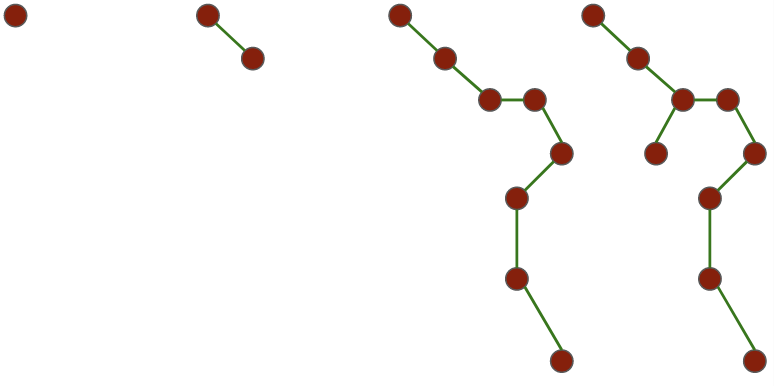
\includegraphics[height=2.7cm]{euler-a}
                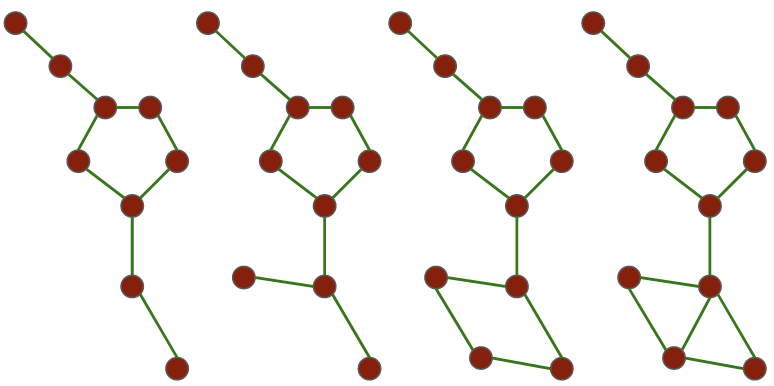
\includegraphics[height=2.7cm]{euler-b}
                \caption{\emph{
                    Steps to build an example constellation (right) starting
                    from a single dot (left).
                    %
                    By the way, this method only helps us build constellations
                    that don't have crossing edges, and each two of whose dots
                    are connected by a path of edges.  Euler's formula only
                    applies to constellations that follow these rules.
                }}
            \end{figure}
            %
            Why is the formula true?  Well, we can build up our constellation
            starting from a single dot.  The single dot follows the formula
            (since there are no regions and no edges, and $0-0+1 = 1$).  And
            each step of building preserves the formula:
            %
            \textbf{either} we connect a new dot to an old dot (so both
            $-\text{Edges}$ and $+\text{Dots}$ change by one, meaning that the
            total stays the same)
            %
            \textbf{or} we connect two old dots to create a new region (so both
            $\text{Regions}$ and $-\text{Edges}$ change by one, meaning that
            the total stays the same).  This logic proves Euler's formula. 

            To wrap up, let's think of a cake as a constellation as shown
            below.  In addition to $n$ outer dots, there are ${n \choose 4}$
            inner dots, because from each inner dot emanate $4$ rays pointing
            toward $4$ outer dots.  By similar logic, the number of edges is $n
            + 2{n\choose 2}/2 + 4{n \choose 4}/2$, since there are $n$ outer
            arcs (green), $2{n\choose 2}$ straight-half edges (blue) between
            outer dots, and $4$ half-edges (orange) emanating from each of
            ${n\choose 4}$ inner dots.
            %
            \begin{figure}[h!]
                \centering
                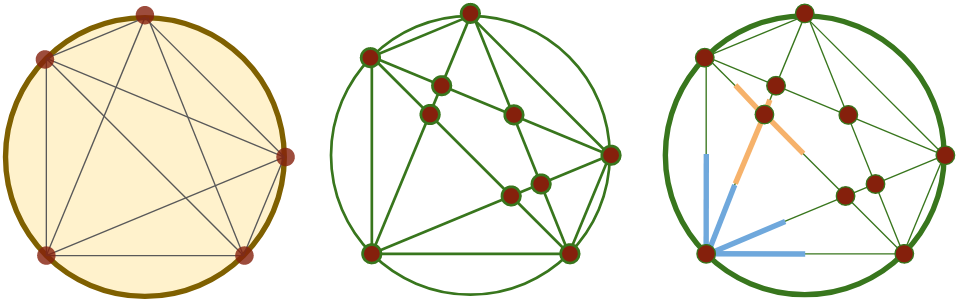
\includegraphics[height=3cm]{count}
                \caption{\emph{
                    We can think of a cake (left)
                    as a constellation (middle) by adding inner dots.
                    We can count the half-edges of the constellation (right) 
                    by binning them into three groups: the outer arcs (green),
                    the straight half-edges between outer dots (blue), and the
                    straight half-edges emanating from inner dots (orange).
                }}
            \end{figure}

            Putting all the pieces together, we find that
            $
                \text{Regions} = 1 + \text{Edges} - \text{Dots}
                               = 1 + {n\choose 2} + {n\choose 4}
            $.  We can simplify this by using the facts that $1={n-1 \choose
            0}$ and ${n \choose k} = {n-1 \choose k-1} + {n-1 \choose k}$:
            \begin{align*}
                \text{Regions}
                              = {n-1 \choose 0}
                              + {n-1 \choose 1}
                              + {n-1 \choose 2}
                              + {n-1 \choose 3}
                              + {n-1 \choose 4}
            \end{align*}
            %
            Since ${n-1\choose 0} + \cdots + {n-1\choose k} = 2^{n-1}$ as long
            as $k\leq n-1$, this looks like powers of two as long as $n\leq 5$.  
            %
            So we have solved the mystery.  With $n$ people, the number $p(n)$
            of pieces equals the number of subsets of $n-1$ people with at most
            $4$ members.    
 
    \chapter{Learning to Classify}
        \section{What is Learning?}
            Today, we'll analyze machines that learn to classify images into
            two possible buckets such as Cow and Dog.
            %Our discussion extends to more complicated situations, but we'll
            %focus on the simple case.  
            To benefit from math, we need a precise set-up.  What do we mean
            by ``learning to classify''?

            Say $\Xx$ contains all possible images and
            $\Yy=\{\text{Cow},\text{Dog}\}$ is the set of buckets.  We posit a
            probability distribution $\Dd$ over $\Xx \times \Yy$ that says
            which pairs $(x,y)\in \Xx\times \Yy$ are more likely and which are
            less likely.  For instance: we might have $\sdia{cow-a},
            \sdia{cow-d},\cdots \in \Xx$, and $\Dd$ might say that
            %
            $(\sdia{cow-a}, \text{Cow})$ is more likely to occur in nature than 
            $(\sdia{cow-d}, \text{Cow})$, which is more likely to occur than
            $(\sdia{cow-d}, \text{Dog})$, which in turn is more likely than
            $(\sdia{cow-a}, \text{Dog})$.

            A \textbf{classifier} is then a function from images to
            buckets, that is, some $f\in \Yy^{\Xx}$.  By \textbf{learning}, we
            mean acquiring information about $\Dd$ from ``training samples''
            $\Ss \in (\Xx\times\Yy)^N$ drawn independently from $\Dd$.  So
            ``learning to classify'' means mapping $\Ss$s to $f$s.  In
            particular, an \textbf{algorithm} is a function
            $\Ll:(\Xx\times\Yy)^N\to \Yy^{\Xx}$.\footnote{ 
                By the way, we don't have to know $\Dd$ in order to apply our
                theory; we just named it in order to reason about it.
                %We'd
                %like our machine to learn by pondering finitely many sample
                %pairs drawn from $\Dd$.
            }

            Instead of considering all possible classifiers, we usually limit
            ourselves to some subset $\Hh \subseteq \Yy^{\Xx}$ of especially
            nice, ``candidate'' classifiers.
            %
            As an example, $\Hh$ might have just three elements:
            \begin{align*}
                \Hh = \{
                    &\text{always say Cow}, \\
                    &\text{say Cow if $x$ is brown on average
                        and otherwise say Dog}, \\
                    &\text{say Cow if
                        $x \in \{\sdia{cow-b}, \sdia{cow-c}, \sdia{cow-e}\}$
                        and otherwise say Dog}
                \}
            \end{align*}
            In practice, $\Hh$ might actually be a much bigger set of neural
            networks.
            %
            \begin{figure}[h!]
                \centering
                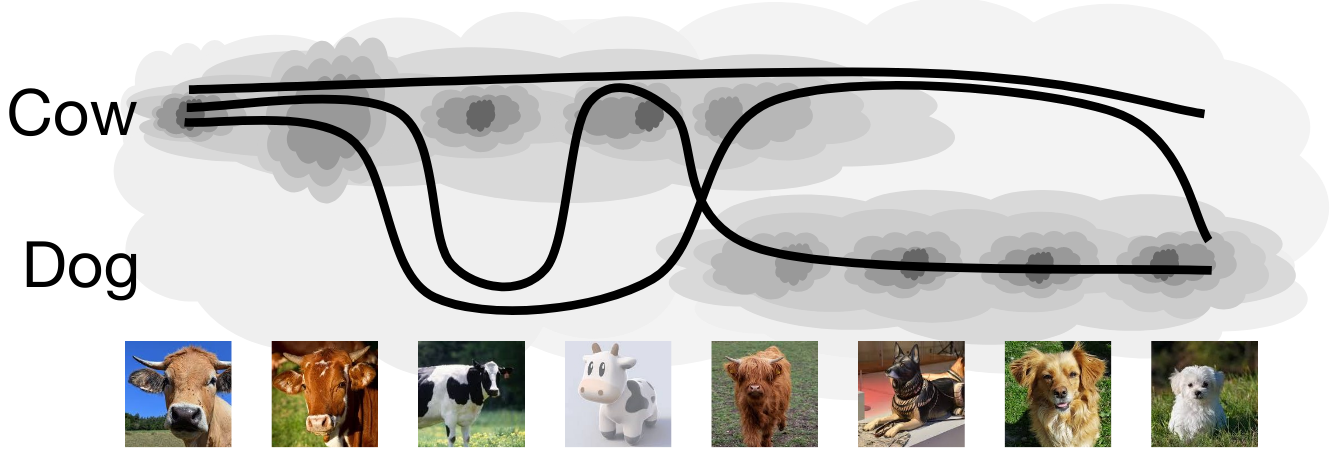
\includegraphics[height=3cm]{hd}
                \caption{\emph{
                    A cartoon of $\Dd$ (clouds) and $\Hh$ (curves) with
                    the $\Xx$ axis horizontal and the $\Yy$ axis vertical. 
                }}
            \end{figure}

            An algorithm $\Ll$ is good when $\Ll(\Ss)$ accurately classifies
            images freshly drawn from $\Dd$.  Notice that this is different
            from merely asking that $\Ll(\Ss)$ accurately classifies the
            elements of $\Ss$!  To notate this difference, we define the
            \textbf{out-error} and \textbf{in-error} (also called the test and
            train errors) of a candidate $f \in \Hh$
            as
            $$
                \Ee_{\text{out}}(f) = \PP_{(x,y)\sim\Dd}   
                                        \left[
                                            f(x) \neq y
                                        \right]
                ~~~~~~~~~~
                \Ee_{\text{in},\Ss}(f) = \PP_{(x,y)\sim\Ss}   
                                       \left[
                                           f(x) \neq y
                                       \right]
            $$
            Likewise, the out- and in-errors of a algorithm are
            $
                \Ee_{\cdots}(\Ll) = \Ee_{\cdots}(\Ll(\Ss)) 
            $ where $\Ss\sim\Dd$.

            We hope $\Ee_{\text{out}}$ is low, but we don't know
            $\Ee_{\text{out}}$: from $\Ss$, we can directly calculate only
            $\Ee_{\text{in},\Ss}$.  Intuiting that
            $ 
                \Ee_{\text{gap},\Ss} = \Ee_{\text{out}} - \Ee_{\text{in},\Ss}
            $ 
            tends to be small, we might design $\Ll$ to minimize $\Ee_{\text{in},\Ss}$.
            That is, $\Ll$ computes $\Ee_{\text{in},\Ss}(f)$ for
            each $f\in \Hh$, then (breaking ties arbitrarily) to settle on an
            $f$ with the least $\Ee_{\text{in},\Ss}$.
            %This $\Ll$ is called
            %\textbf{ERM};
            %its variants dominate modern
            %machine learning.
            
            This $\Ll$ will work when $\Ee_{\text{gap},\Ss}$ is small.
            But is $\Ee_{\text{gap},\Ss}$ actually small?  In particular, if
            $\Ll(\Ss)$ accurately classifies its training samples, will it also
            accurately classify test samples it has never before seen?

            Sometimes, the answer is \textbf{yes}.
                If there is $1$ candidate $f\in \Hh$ and a thousand
                datapoints, then $\Ee_{\cdots}(\Ll) = \Ee_{\cdots}(f)$, and
                $\Ee_{\text{in},\Ss}(f)$ will very probably be very close to
                $\Ee_{\text{out}}(f)$.  A technical reason for this is that
                $\Ll(\Ss)$ and $\Ss$ are independent, and we may apply the law
                of large numbers.  It's as if we roll a fair die a thousand
                times: we'd expect about a sixth of the rolls to land on
                \epsdice{5}.

            Other times, the answer is \textbf{no}.
                If every possible classifier is a candidate (so $\Hh$ is very
                infinite) and only a few datapoints, then for any training
                sequence $\Ss$, many candidates will perfectly classify the
                training samples.  Say that $\Ll$ breaks ties 
                by settling on
                $$
                    f(x) = \text{say Cow if $(x,\text{Cow}) \in \Ss$;
                            otherwise, say Dog}
                $$
                The problem (assuming each image appears with negligible chance
                and that Cows occur with non-negligible chance) is $f$ will
                misclassify every fresh image of a Cow as a Dog, so it will
                have a huge out-error!  It's as if we do a trillion experiments
                where in each experiment we roll a fair die a thousand times:
                in any one experiment, we'd expect about a sixth of the rolls
                to land on \epsdice{5}, but if we focus on the experiment that
                has the most \epsdice{5}s (which is like focusing on the
                hypotheses that do the best on the training data), we are
                likely to focus on an outlier that has disproportionately many
                \epsdice{5}s!

            These two examples illustrate that $\Ll$'s training performance
            generalizes to test time when $\Ll$ uses lots of datapoints to
            select from only a small set of candidates.  
            %
            How do these forces balance, for example if there are a lot of
            candidates and also a lot of datapoints?  Let's find out.

        \section{Is Learning Possible?}
            Let's analyze the case $|\Hh|=1$ more closely.  We write $p$ as
            shorthand for $\Ee_{\text{out}}(f)$; then $\Ee_{\text{in},\Ss}$
            counts the fraction of heads that appear in $N$ independent flips
            of a coin that has chance $p$ of landing heads.  Intuitively
            $\Ee_{\text{in},\Ss}$ will usually be close to $p$ when $N$ is big.
            Let's make ``usually'', ``close to'', and ``big''  precise.

            \begin{figure}[h!]
                \centering
                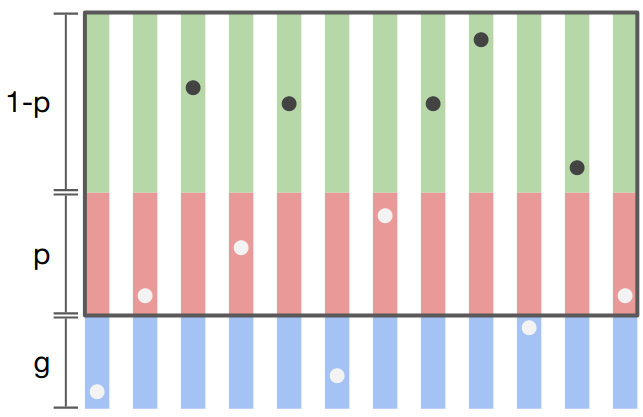
\includegraphics[height=4cm]{chernoff}
                \caption{\emph{
                    We randomly select points on $N$ vertical sticks.  Each
                    stick has three parts: \textbf{green} with length $1-p$,
                    \textbf{red} with length $p$, and \textbf{blue} with length
                    $g$.  We call non-blue points \textbf{boxed} and non-green
                    points \textbf{hollow}.
                }}
            \end{figure}

            We'll switch viewpoints: flipping a coin is like choosing a boxed
            point on a stick where green means tails and red means heads.
            %
            We'll show that probably at most $M_0 = (p+g)N$ heads
            appear.  That is, we want to show --- given that all points are
            boxed --- that probably at most $M_0$ points are red. 
            %
            For any $M\geq M_0$:
            \begin{align*}
                    & ~ \PP[\text{$M$ are red $\mid$ all are boxed}] \\
                  = & ~ \PP[\text{$M$ are red and all are boxed}] ~/~ 
                        \PP[\text{all are boxed}]  \\
                  = & ~ \PP[\text{$M$ are hollow}] \cdot
                        \PP[\text{all hollows are red $\mid$ $M$ are hollow}] ~/~
                        \PP[\text{all are boxed}] \\
                  = & ~ \PP[\text{$M$ are hollow}] \cdot (1+g/p)^{-M} ~/~ (1+g)^{-N}  \\
                \leq& ~ \PP[\text{$M$ are hollow}] \cdot (1+g/p)^{-M_0} ~/~ (1+g)^{-N} 
            \end{align*}
            Since the above holds for all $M\geq M_0$, we conclude:
            \begin{align*}
                ~   & ~ \PP[\text{at least $M_0$ are red $\mid$ all are boxed}] & \\
                \leq& ~ \PP[\text{at least $M_0$ are hollow}] \cdot (1+g/p)^{-M_0} / (1+g)^{-N} \\ 
                \leq& ~ (1+g/p)^{-M_0} / (1+g)^{-N}             & \text{probabilities are at most $1$} \\
                \leq& ~ \exp(-M_0 g/p) \exp(Ng)                 & \text{$1+x\leq \exp(x)$} \\ 
                =   & ~ \exp(-(p+g)N g/p + Ng)                  & \text{substitute $M_0=(p+g)N$} \\ 
                =   & ~                          \exp(-Ng^2/p)  & \text{simplify}                \\ 
                \leq& ~ \exp(-Ng^2)                             & \text{probabilities are at most $1$}
            \end{align*}
            This is the \textbf{Chernoff bound} for coin flips.\footnote{
                There are lots of versions of this bound.  Google up 
                ``multiplicative Chernoff bound'' or ``Bernstein inequality''
                for some fun examples!
            }

            What have we learned?  We have learned that if we flip a fair coin
            $N$ times, the odds of deviating by more than $1\%$ from the
            expected value of $50\%$ heads decays very quickly with $N$!  Tying
            back to learning, if hypothesis $f$ accurately classifies
            $80\%$ of a large training set ($E_{\text{in},\Ss}=0.2$), then $f$
            will probably accurately classify about $80\%$ of its test set
            ($E_{\text{out}}\approx 0.2$).  For example, if there are $N=300$
            training points, then the odds of $f$ suffering less than $70\%$
            test accuracy are less than $$ \exp(-Ng^2) = \exp(-300 \cdot
            10\%^2) \approx 5.0\% $$

            Notice the exponential dependence on $N$!  Intuitively, exponential
            dependencies are strong dependencies.  For example, if we add
            $10^4$ to $N$, then we get
            $$
                \exp(-Ng^2) = \exp(-400 \cdot 10\%^2) \approx 1.8\%
            $$
            And if we add yet another $10^4$ to $N$, then we get
            $$
                \exp(-Ng^2) = \exp(-500 \cdot 1\%^2) \approx 0.67\%
            $$
            The chance of an inacceptable test accuracy decays
            quickly with $N$.  Data is useful!

            We can likewise play with $g$ instead of $N$.  Since $g$ is squared in the
            formula, it can have a huge effect on the probability of success.
            What if we think that a generalization gap of $g=10\%$ test
            accuracy is too much?  For $g=8\%$, we find:
            $$
                \exp(-Ng^2) = \exp(-500 \cdot 6\%^2) \approx 4.1\%
            $$
            For $g=6\%$:
            $$
                \exp(-Ng^2) = \exp(-500 \cdot 6\%^2) \approx 16\%
            $$
            The chance of an inacceptable test accuracy increases very quickly
            quickly as our notion of acceptability becomes more stringent.
            Tolerance is useful!


            Now, instead of trying different values of $g$, we might want to 
            solve for $g$ in terms of a probability of failure that we name
            $\delta$.  We find that with probability at most $\delta$ will the
            generalization gap exceed $\sqrt{\log(1/\delta)/N}$.  Call this
            $\Gg(\delta)$.
  
        \section{Multiple candidates}
            What if $\Hh$ contains multiple (say, $H$ many) candidates?
            Well, each candidate $f\in \Hh$ has
            $
                \Ee_{\text{gap},\Ss}(f) \geq \Gg(\delta/H)
            $
            with probability at most $\delta/|\Hh|$.  Therefore, the chance
            that some $f\in \Hh$ has
            $
                \Ee_{\text{gap},\Ss}(\Ll) \geq \Gg(\delta/H)
            $
            is at most $H$ times $\delta/H$.  In sum,
            with probability at least $1-\delta$ the gap will be small:
            $$
                \Ee_{\text{gap},\Ss}(\Ll)
                    \leq \max_{f\in\Hh} \Ee_{\text{gap}, \Ss}(f)
                    < \Gg(\delta/H)
                    = \sqrt{\log(H/\delta)/N}
            $$

            What we have shown is that, if our algorithm $\Ll$ selects from among
            a finite number of candidates, then learning is possible: the
            more data points we have, the smaller will be the generalization
            gap bound $\Gg(\delta/H)$.

            Here's an example.  Suppose we train a neural net that has $10^3$
            parameters, each a floating point number.  Since there are at most
            $2^{32}$ possible floating point numbers, $H$ is at most
            $2^{32\cdot 10^3}$.  If we train on $10^6$ images, then with
            probability $99.99\%=1-10^{-4}$, the generalization gap is less
            than
            $$
                \sqrt{\log(2^{32\cdot 10^3}/10^{-4})/10^6}
                \approx 9.8\%
                \approx 10\%
            $$
            So if after training, the neural net's training accuracy is $80\%$,
            we can expect its testing accuracy to be at least $70\%$.
            We proved this without knowing $\Dd$; we used simply that $\Dd$
            exists at all!  Ain't that cool?

    %\chapter{Structure in $\Hh$}
    %    \section{Symmetrization}
    %    \section{The Vapnik Chervonenkis Dimension}

    %\chapter{Structure in $\Dd$}
    %    \section{Rademacher Complexity}
    %    \section{Margin Bounds}

    %\chapter{Structure in $\Ll$}
    %    \section{Privacy and Generalization}
    %    \section{The Akaike Information Criterion and its Cousins}

    %\chapter{Frame Conditions and Independence}
    %    \section{Simplicity and Subjectivity}
    %    \section{Independence in Practice?}

    %\newpage
    %\chapter*{Helping Handout: Binomial Coefficients ${n \choose k}$}
    %    How many ways can we select $k$ people out of $n$ people?
    %    For example,
    %    there is just $1$ way to choose a pair ($k=2$) from among $n=2$ people.
    %    There are $3$ pairs among $n=3$ people.
    %    And there are $6$ pairs among $n=4$ people.
    %    We write the answer to this question as ${n\choose k}$; so
    %    ${4\choose 2} = 6$. 
    %    
    %    While ${n\choose k}$ counts size-$k$ subsets, so that picking Alice 
    %    and Bob is the same as picking Bob and Alice, we might want to count
    %    ordered subsets.
    %    How about if we want to order $k=4$ people out of $n=10$ people?
    %    Well, there are $10$ ways to select the first person,
    %                     $9$ ways to select the second person,
    %                     $8$ ways to select the third person, and
    %                     $7$ ways to select the fourth person.
    %    So the answer is $10\cdot 9\cdot 8\cdot 7$.
    %    But each size-$k$ unordered subset corresponds to
    %    $4\cdot 3\cdot 2\cdot 1$ ordered subsets.  So we conclude that
    %    $$
    %        {10\choose 4} = \frac{10\cdot 9\cdot 8\cdot 7}{4\cdot 3\cdot 2\cdot 1} 
    %    $$

    %    Notice that ${n \choose 0} = 1$, since there is always exactly one way
    %    to choose none of the $n$ people.
    %    %
    %    Also, when $n$ is positive, ${n\choose k} = {n-1\choose k-1} +
    %    {n\choose k-1}$, since to choose $k$ folks from among a group of $n-1$
    %    students and $1$ teacher, we can \textbf{either} choose $k$ students
    %    and leave out the teacher \textbf{or} choose $k-1$ students and also
    %    the teacher.
    %    %
    %    Another neat fact is that
    %    $
    %        {n\choose 0} + {n\choose 1} + {n\choose 2} + \cdots + {n\choose k}
    %        = 2^n
    %    $
    %    as long as $n\leq k$.  This is because that sum
    %    counts the number of ways to choose some subset of size at
    %    most $k$ from among $n$ people.  

    %\chapter*{Helping Handout: Asymptotics}

    %\newpage
    %\chapter*{Helping Handout: Probability}
    %    How can we model the notion of \textbf{chance} using math?
    %    For example, we might have a set $\Xx=[0\,\text{cm}, 50\,\text{cm}]$ of
    %    possible daily rainfall levels.  Intuitively, there is zero chance that
    %    any particular positive rainfall like $6.28318\cdots\,\text{cm}$ will
    %    occur today.  But we'd say there is some chance that the rainfall will
    %    fall within, say, $[6.2\,\text{cm}, 6.3\,\text{cm}]$.
    %    %
    %    Thus, in order to treat $\Xx$ probabilistically, we want to assign to
    %    each interval $I \subseteq \Xx$ a nonnegative number $\PP(I)$ that
    %    tells us the chance that rainfall will fall within $I$.  In order for
    %    this bunch of numbers to make sense, we demand $\PP(\Xx)=1$ and that,
    %    whenever a bunch of intervals $I_0, I_1, \cdots$ partition a bigger
    %    interval $J$, then $\PP(I_0) + \PP(I_1) + \cdots = \PP(J)$.
    %    By the way, it is convenient to think of $\PP$ as defined on unions of
    %    disjoint intervals instead of intervals.

    %    In general, a \textbf{probability distribution} on a set $\Xx$ is a
    %    bunch of ``generalized unions-of-intervals'' of ``events'' that are subsets of $\Xx$,
    %    each labeled by a nonnegative number, that
    %    follows the above demands.  Precisely, the data is: a collection $\Ii
    %    \subseteq 2^\Xx$ of subsets of $\Xx$ and a function $\PP:\Ii\to [0,
    %    1]$, such that the following are well-defined and true whenever $I,
    %    I_0, I_1, \cdots \in \Ii$.
    %    $$ 
    %        \PP(\Xx - I) + \PP(I) = \PP(\Xx) = 1 
    %    $$
    %    and
    %    $$
    %        \PP(I_0) + \PP(I_1) + \cdots = \PP(I_0 \cup I_1 \cup \cdots)
    %        ~~~~~
    %        \text{when the $I$'s are disjoint}
    %    $$

    %    One technique to understand complicated events is to break them up
    %    into simpler events.  For example, it is intuitive that the chance that
    %    a coin lands heads while a die lands sixes is related to the separate
    %    chances that a coin lands heads and that a die lands sixes.  In particular,
    %    we expect heads to occur $1/2$ of the time and sixes to occur $1/6$ of
    %    the time, and thus both together to occur $(1/2) \cdot (1/6) = 1/12$ of
    %    the time.  When simple events compose this way, we call them
    %    \textbf{independent}:
    %    $$
    %        \PP(I_0 \cap I_1 \cap \cdots) = \PP(I_0) \cdot \PP(I_1) \cdot \cdots
    %        ~~~~~
    %        \text{when $I_0, I_1, \cdots$ are independent} 
    %    $$
    %    Events aren't always independent though.  In general, we may define
    %    symbols $\PP(I | J)$ for the \textbf{conditional probability} that $I$
    %    happens assuming that $J$ happens:
    %    $$
    %        \PP(I \cap J) = \PP(I | J)\cdot \PP(J)
    %    $$
    %    There is exactly one choice for $\PP(I|J)$ when $\PP(J)\neq 0$.
    %    we may choose $\PP(I|J)=\PP(I)$ exactly when $I, J$ are independent.
    %    %
    %    Conditional probabilities formalize ``what if'' questions:
    %    For example, what is the chance that of $\geq 2\,\text{cm}$ of rain
    %    given $\geq 1\,\text{cm}$ of rain?  

    %    \section*{Monty Hall}
    %        Here's a practice example.  Imagine three boxes, exactly
    %        one of which contains a prize.  We don't know which.
    %        We play a game that has three steps: First, we pick a box.  Next, a
    %        gameshow host removes one of the empty boxes that isn't the box we
    %        picked.  Finally, we are allowed to pick one of the two remaining
    %        boxes; it will either be our original box, or a different box.  If
    %        this final pick contains the prize, then we win.

    %        Here are three strategies we might use:
    %        \textbf{stay} --- we pick the original box; or
    %        \textbf{swap} --- we pick the different box; or
    %        \textbf{flip} --- based on a flip of a fair coin, we pick the original or different box.

    %        The \textbf{stay} strategy has a $1/3$ chance of winning, since 
    %        playing the game with this strategy leads us to choose the prize
    %        box as much as one empty box as much as the other empty box.

    %        The \textbf{flip} strategy has a $1/2$ chance of winning, since 
    %        playing the game with this strategy leads us to choose the prize
    %        box as much as the empty remaining box.

    %        And $\PP_{\textbf{flip}}(\text{win})$ is the average of 
    %        $\PP_{\textbf{stay}}(\text{win})$ and
    %        $\PP_{\textbf{swap}}(\text{win})$.
    %        Therefore, the \textbf{swap} strategy has a $2/3$ chance of
    %        winning.  It is by far the best.

    %\chapter*{Helping Handout: Vectors and Covectors}
    
\end{document}


